% Use only LaTeX2e, calling the article.cls class and 12-point type.
%testcommit

\documentclass[12pt]{article}

% Users of the {thebibliography} environment or BibTeX should use the
% scicite.sty package, downloadable from *Science* at
% www.sciencemag.org/about/authors/prep/TeX_help/ .
% This package should properly format in-text
% reference calls and reference-list numbers.


%\usepackage{scicite}
\usepackage{multirow}
\usepackage{graphicx}
\usepackage{amsmath,array,mathtools}
\usepackage{color,soul}
\usepackage[toc,page]{appendix}
\usepackage[symbol]{footmisc}
\usepackage[hyphens]{url}
\usepackage[table]{xcolor}
\usepackage{hhline}
% Use times if you have the font installed; otherwise, comment out the
% following line.

\newcommand{\red}[1]{\textcolor{black}{#1}}

\usepackage{times}

% The preamble here sets up a lot of new/revised commands and
% environments.  It's annoying, but please do *not* try to strip these
% out into a separate .sty file (which could lead to the loss of some
% information when we convert the file to other formats).  Instead, keep
% them in the preamble of your main LaTeX source file.


% The following parameters seem to provide a reasonable page setup.

\topmargin 0.0cm
\oddsidemargin 0.2cm
\textwidth 16cm 
\textheight 21cm
\footskip 1.0cm


%The next command sets up an environment for the abstract to your paper.

\newenvironment{sciabstract}{%
\begin{quote} \bf}
{\end{quote}}


% If your reference list includes text notes as well as references,
% include the following line; otherwise, comment it out.

\renewcommand\refname{References and Notes}

% The following lines set up an environment for the last note in the
% reference list, which commonly includes acknowledgments of funding,
% help, etc.  It's intended for users of BibTeX or the {thebibliography}
% environment.  Users who are hand-coding their references at the end
% using a list environment such as {enumerate} can simply add another
% item at the end, and it will be numbered automatically.

\newcounter{lastnote}
\newenvironment{scilastnote}{%
\setcounter{lastnote}{\value{enumiv}}%
\addtocounter{lastnote}{+1}%
\begin{list}%
{\arabic{lastnote}.}
{\setlength{\leftmargin}{.22in}}
{\setlength{\labelsep}{.5em}}}
{\end{list}}



\title{Energy and Time Determine Scaling in \\Biological and Computer Designs} 


\author
{Melanie Moses,$^{1,2,3\ast}$ George Bezerra,$^{1}$ \\Benjamin Edwards,$^{1}$ James Brown,$^{2,3}$ Stephanie Forrest$^{1,2,3}$\\
\\
\normalsize{$^{1}$Department of Computer Science}\\
\normalsize{University of New Mexico, Albuquerque, NM, USA.}\\
\normalsize{$^{2}$Department of Biology}\\
\normalsize{The University of New Mexico, Albuquerque, NM, USA.}\\
\\
\normalsize{$^{3}$The Santa Fe Institute, Santa Fe, NM, USA.}\\
\\
\normalsize{$^\ast$To whom correspondence should be addressed}\\
\normalsize{E-mail: melaniem@cs.unm.edu}\\
\normalsize{Address: Department of Computer Science}\\
\normalsize{1 University of New Mexico, Albuquerque, NM USA}\\
\normalsize{Phone: 505-277-3112}\\
}






%%%%%%%%%%%%%%%%% END OF PREAMBLE %%%%%%%%%%%%%%%%

\newcommand\T{\rule{0pt}{3ex}}       % Top strut
\newcommand\B{\rule[-1.2ex]{0pt}{0pt}} % Bottom strut


\begin{document} 

\newcounter{casenum}
\newenvironment{caseof}{\setcounter{casenum}{1}}{\vskip.5\baselineskip}
\newcommand{\case}[2]{\vskip.5\baselineskip\par\noindent {\bfseries Case
\arabic{casenum}:} #1: #2\addtocounter{casenum}{1}}

% Double-space the manuscript.

\baselineskip24pt

% Make the title.

\maketitle 


\newpage


\centerline{\Large{\bf Abstract}}

\begin{sciabstract}

  Metabolic rate in animals and power consumption in computers are analogous
  quantities that scale similarly with size.  We analyze vascular systems of
  mammals and on-chip networks of microprocessors, where natural selection
  and human engineering respectively have produced systems that minimize both energy dissipation
  and delivery times.   
  Using a simple network model that simultaneously minimizes energy
  and time, our analysis explains empirically observed trends in the scaling of metabolic rate in mammals  and power consumption and performance in microprocessors across several orders of magnitude
  in size.  Just as
  the evolutionary transitions from unicellular to multicellular animals in biology are associated with shifts in
  metabolic scaling, our model suggests that the scaling of power and performance will change
  as computer designs transition to decentralized multi-core and
  distributed cyber-physical systems. More generally, a single energy-time minimization principle may govern the design of many complex systems that process energy, materials, and information. 

\end{sciabstract}

\newpage

\section{Introduction}
\label{sec:intro}

Both organisms and computers have evolved from relatively simple beginnings
into complex systems that vary by orders of magnitude in size and number of
components. Evolution, by natural selection in organisms and by human
engineering in computers, required critical features of architecture and
function to be scaled up as size and complexity increased. In biology,
Kleiber's law describes empirically how metabolic rate and many
other traits, such as lifespan, heart rate, and number of offspring, scale with body
size \cite{kleiber47}.  Similarly, computer architecture has Moore's law to
describe scaling of transistor density and performance \cite{moore98}, Koomey's
law for the energy cost per computation \cite{koomey11}, and Rent's rule for
the external communication per logic block \cite{christie00}.

We posit that these empirical patterns originate from a common principle:
Networks that deliver resources are optimized to reduce energy dissipation and
increase flow rates, expressed here as minimizing the energy-time product. That
is, both living systems and computer chips are designed to maximize the rate at
which resources are delivered to terminal nodes of a network and to minimize
the energy dissipated as it is delivered and processed.  For example, in biology the vascular network of mammals supplies oxygen and nutrients to every cell, fueling metabolism for
maintenance, growth and reproduction.  Since energy is a limited resource, we
assume that mammals are selected to minimize the time spent and energy dissipated as oxygen is delivered through the network \cite{west97} and processed to produce ATP in the mitochondria. Similarly, computation in microprocessors relies on a
network of microscopic wires that transmits bits of information between
transistors on a chip. This network is designed to deliver the maximum information
flow at the lowest possible energy cost.

Here, we model mammals as composed of nodes (regions of tissue) that process oxygen
delivered via a hierarchical vascular network, and we model
microprocessors as composed of nodes (transistors that perform computation) that communicate
bits over a network of wires.  As each system scales up in size,
our model identifies network designs that minimize 1) the rate at which resources are delivered by the network and
processed in the nodes; and 2) the energy dissipated during these processes.
Despite the obvious differences between animals and chips, we present a
general model and derive energy and time scaling relations from physical
principles applicable to each system. Using these relations, we express the
optimal network design as a trade-off between energy cost and processing speed. \red{This energy-time minimization model is consistent with shifts across the major
evolutionary transitions,
such as the transition from protists to
multicellular animals and the transition from single- to multi-core
computer chips.
It also points to likely future trajectories of the evolution of
computer architecture and to possible extensions of metabolic scaling
theory to account for sociality.}


\red{Previous biological scaling models have sought either to minimize energy dissipation, e.g.,~\cite{west97} or to maximize resource delivery rate~\cite{banavar10}, but they have
not formalized the trade-offs between these goals.  By simultaneously considering energy and time minimization, our analysis
helps to explain how nature and engineering are able to produce designs that
approach pareto-optimality along the energy-time trade-off, a question investigated extensively in computer architecture, e.g.,~\cite{horowitz2005scaling, azizi2010energy}. Thus, biological
evolution has produced mammals ranging in size from mice to elephants, rather
than converging on a single optimal size, and computer engineers have designed processors with thousands to
billions of transistors, each of which fills a specific computational niche.}

In the rest of the paper, we present the unified time-energy minimization model
(Section \ref{sec:unified-model}) and its assumptions (Section ~\ref{sec:assumptions}).  We then use the model to derive a
series of predictions about how time and energy scale with system size, first
for mammals (Sections \ref{sec:mammals} and \ref{sec:bio-predictions}) and then for microprocessors (Section
\ref{sec:computers}). We discuss new insights into previously analyzed
scaling relationships in biology that we gain from the time-energy minimization
framework, and we test our scaling predictions with empirical power and performance
data on computer chips.  Finally, in Section \ref{sec:discussion}  we discuss
the implications of these results for evolutionary transitions in nature and
engineering.

\begin{figure}[!h]
\centering
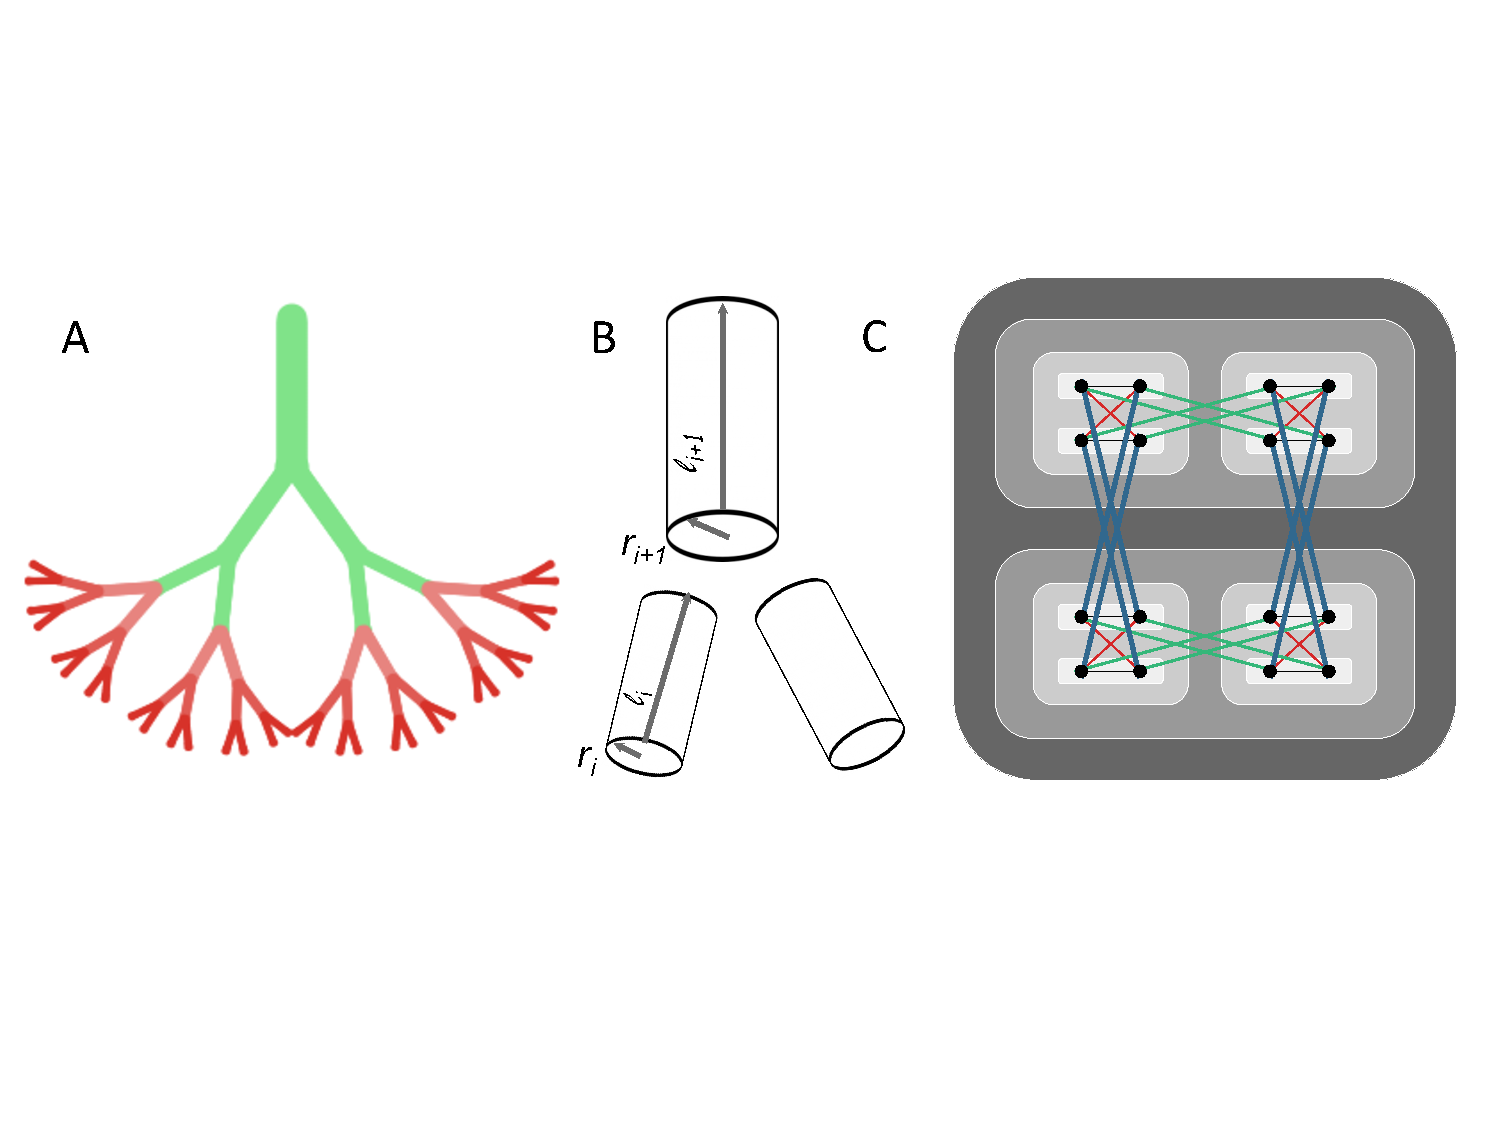
\includegraphics[width=\textwidth]{Figures/Figure1Draft4.pdf}
\label{fig:firstfig}

\caption{Idealized branching models in biology (Panel A) and computers
  (Panel C). Panel A shows a cardiovascular tree with branching factor $\lambda
  = 2$, $H = 5$ hierarchical branchings, and $N = 32$ terminal
  branches at level 0 that represent capillaries. \red{Panel B shows the radius and length of successive branches: $D_r$ defines the relative radius and $D_l$ defines the relative length of pipe or wire between successive hierarchical levels ($i$ and $i+1$) in both biology (Panel A) and computers (Panel C). Panel C shows the semi-hierarchical branching of logic wires on a computer chip. Each module within a
  hierarchical level is shaded the same color. The purple, red, green and blue wires cross 0, 1, 2 and 3 modules respectively. The wire lengths and widths increase as they cross more levels according to $D_l$ and $D_r$. $D_w$ defines the number of wires, determined by the ratio of internal (intra-module) communication per
  node to external (inter-module) communication per node. Here $D_w = 2$ so that a node is connected to all nodes within a module (in this case only 1) by a purple wire, 1/2 of the nodes in the next hierarchical level by red wires, 1/4 of the nodes in the next level by green wires, and 1/8 of the nodes in the next level by blue wires.}}

\end{figure}
\section{Unified Model of Network Scaling}
\label{sec:unified-model}


Vascular systems are hierarchical branching networks where blood vessels
(pipes) become thicker and longer through the hierarchy from the capillaries
to the aorta. Similarly, microprocessor chips are organized hierarchically into
a nested structure of modules and submodules, where wires become longer and
thicker as the hierarchical level of a module increases
(Figure~\ref{fig:firstfig}).  These wires are organized into metal
layers, where short, thin wires are routed on the lowest layers, and long,
thick wires are placed on the top layers. We model the scaling of length ($l$)
and thickness ($r$) of both pipes and wires as:

\begin{equation}
l_i = l_0 \lambda^{\frac{i}{D_l}}
\end{equation}

\noindent and

\begin{equation}
  r_i = r_0 \lambda^{\frac{i}{D_r}},
\label{eq:rscaling}
\end{equation}

\noindent where $i$ is the hierarchical level of a branch or module, $\lambda$
is the branching factor, and $D_l$ and $D_r$ are the length and thickness
dimensions. This model resembles the hierarchical pipe model of vascular
systems proposed in \cite{west97}, where $\lambda^{\frac{1}{D_r}}$ and
$\lambda^{\frac{1}{D_l}}$ correspond to  $\beta$ and $\gamma$
respectively in~\cite{west97} (note that in~\cite{west97}, the aorta or top of the network is
labelled as level 0, while here the smallest branches, the capillaries, are
labelled as level 0).

In vascular networks, $r$ represents the radius of cylindrical pipes, and in
computer interconnect, $r$ represents the width of wires with aspect ratio 1.
$D_r$ describes the relative radius of pipes between successive hierarchical
levels.  The smallest edges occur at $i = 0$, and have constant radius, $r_0$,
but length, $l_0$, that scales with system size~\cite{banavar10}. 

The length parameter $D_l$ is determined by the spatial dimension occupied by the
nodes of the network~\cite{mandelbrot83}.  For chips, $D_l = 2$, since
transistors are placed on a single two-dimensional layer~\cite{donath81}. For
three-dimensional organisms,  $D_l = 3$. Because the length of a
vessel defines the radius of a 3-dimensional volume of tissue supplied
by that vessel, each successive vessel in the hierarchy also scales
according to Eq. 1 with $D_l = 3$~\cite{west97, banavar10}. Similarly,
the length of each successive wire on a 2-dimensional chip defines the
area to which that wire delivers signals~\cite{moses08}. Thus, in the simplest networks that efficiently deliver resources homogeneously throughout a volume or area, $D_l$ describes both the relative length of pipe between successive hierarchical levels and the physical
dimension of the system. For example in \red{Figure \ref{fig:firstfig} C}, where \red{$\lambda = 2$ and $D_l = 2$, wires are $2^{1/2} = 1.41$} times longer when they connect to successively higher modules in the hierarchy.

Digital circuits scale in a third way beyond length and radius, which
has no direct analog in mammalian cardiovascular networks. Digital circuits are partially \emph{decentralized}, with networks that connect multiple sources and destinations, while vascular networks are
centralized, with blood flowing from a single heart. 
In vascular networks, each pipe
branches at each hierarchical level forming a tree structure
(in the simplest case with $\lambda = 2$ forming
a binary tree.) Chips, however, have many connections within each
level of the network, and the number of these connections
varies systematically with the hierarchical level.  
 To account for
this difference, we introduce a new equation, in which the
communication (or number of wires) per module increases with the
hierarchical level as:  

\begin{equation}
  w_i = w_0 \lambda^{\frac{i}{D_w}}
\label{eq:communication}
\end{equation}

\noindent where $D_w$ is the communication dimension and $w_0$ is the average
number of wires per node.  This hierarchical scaling of communication is a
well-known pattern in circuit design called Rent's rule \cite{christie00},
where $p = \frac{1}{D_w}$ is the Rent's exponent.\footnote{Rent's rule is typically
  expressed as $C(n) = kn^p$, where $C_n$ is the external communication of a
  module, $n$ is the size of the module (number of nodes), $k$ is the average
  external communication of a module with size 1, and $p$ is Rent's
  exponent. For a hierarchy with branching factor of $\lambda$, the size of a
  module is given as $n = \lambda^i$, where $i$ is the hierarchical level.
  Therefore, we can rewrite Rent's rule as $c_i = c_0 \times \lambda^{ip}$,
where $c_0 = w_0$ and $p = \frac{1}{D_w}$.} This pattern is not unique to circuits
and has been shown to occur in many biological networks
\cite{reda09,bassett10,meunier2010modular,solee2013evolutionary}.   Vascular systems correspond to a special case where 
$w_i = 1$ for all $i$. 

\subsection{Assumptions of the Unified Model}
\label{sec:assumptions}

Before presenting the model and deriving scaling predictions, we state the
model's assumptions and how they relate to earlier models, both in
computation and biology:

\begin{enumerate}
\item {\bf Time and energy are equally important constraints:} 
  System designs seek to deliver the maximum quantity of
  resource per unit time for the minimum quantity of energy expended. 
  In computer architecture this relationship is expressed as the
  \emph{energy-delay product}, which formalizes the insight that a
  chip that is ten times faster or ten times more energy efficient is
  ten times better ~\cite{horowitz1994low}.   In synchronous systems, clock speed (delay
  between clock ticks) determines the maximum rate at which the system can compute.

\item {\bf Steady state}: Resource supply matches processing
  demand~\cite{banavar2002supply, banavar10}.  That is, the network supplies resources continually
  to the nodes and is always filled to capacity.  This avoids network
  delays and the need to store resources in the system. Specifically,

  \begin{enumerate}

\item System designs balance network delivery rates with node processing
  speeds, so that resources are delivered at exactly the same rate that they
  are processed.

\item Pipelining: A concept from computer architecture in which resources,
  e.g., computer instructions, leave the source at the same rate that they are
  delivered to the terminal nodes, and the network is always full.  %In the hierarchical networks considered here, the source is the highest branch and the principle holds within every level of the hierarchy.
  Consequently, resources (oxygen molecules or bits) flow through the network continually 
  without bottlenecks, and they do not accumulate at source, sink, or intermediate locations.
  \end{enumerate}

\item {\bf Terminal units and service volumes:} \red{We follow previous scaling
    models of biology, which posit that the service volume (the volume of
    tissue that is supplied by a single terminal unit of the network) increases with
  system size and has a fixed metabolic rate~\cite{west97, banavar10}.}  In contrast to~\cite{west97} we do not assume that terminal branches of the vascular network have fixed size. Following~\cite{banavar10}, we assume that the length ($l_0$) of the terminal branches of the network (e.g., capillaries) is
  proportional to the radius of the service volume.  We also follow
  the assumptions in~\cite{banavar10} that the capillaries have fixed
  radius, and that the speed of flow ($u_0$) through the service volume is
  proportional to its length, so that the rate of arrival of oxygen
  molecules to mitochondria in the service volume is constant across mammals.   In
  chips, transistor size has shrunk over many orders of
  magnitude over the past 50 years.
\red{Similar to the length scaling of the service volume in mammals, the
radius of the isochronic region (the service area) for chips scales
proportionally with decreasing transistor size~\cite{moses08}. Thus,
	service regions are \emph{smaller} in more powerful chips (which have more transistors), but they are \emph{larger} in larger animals. We refer to the service volumes in mammals and the service regions on chips as \emph{nodes}.}
\end{enumerate}

In addition to these general assumptions, we make the following
refinements to accommodate salient differences between biology and computer architecture.
\begin{enumerate}
\item In biology, the energy processed by a node 
  ($E_{node}$) is invariant with system size. That is, as the size of a service volume
  increases with body size, the total amount of energy it processes
  remains constant. We do not make this assumption for chips.

\item Component packing: In chips, we assume that total chip area is constant, and the
  number of transistors ($N$) is the square of the process size, i.e.,
  the length of one side of a transistor. 

\end{enumerate}

\noindent 

In biology it is known that blood flow slows by several orders of magnitude as
it travels from the aorta to the capillaries~\cite{west97}.
Earlier scaling models have generally not characterized this
slowing~\cite{west97, banavar10}, but
our equations include velocity as an explicit term, to highlight where it affects time and energy
scaling. Here we model $D_r$ as constant within an organism so that blood slows continuously from the heart to the capillaries. We also model $D_w$ and $D_l$ as constant. Because rates of blood flow, oxygen delivery, and ATP synthesis can be converted one to another by a simple conversion constant, we treat them interchangeably in our scaling model.

\section{Model Predictions for Mammals and Microprocessors}

We define $E_{net}$ and $T_{net}$ respectively to be the energy dissipated and
the time taken by the network to deliver a fundamental unit of resource to each node.  For
mammals the resource is oxygen (in mammals, carried by a unit volume of
blood), and for computers the resource is a bit of information.
Similarly, we define $E_{node}$ and $T_{node}$ as the energy dissipated and the
time taken by the nodes to process that resource.  For mammals, the node is
the service volume corresponding to a region of tissue supplied by a single
capillary~\cite{banavar10}, which corresponds to a volume of tissue containing a constant number
of mitochondria~\cite{west2002allometric}, the organelles that process oxygen molecules to generate
biologically useful energy in the form of ATP. A node is defined as having a constant
rate of delivery of oxygen and processing of oxygen, but the
volume of a node varies with organism size. 

$E_{net}$ is the energy required to deliver oxygen to the cells (as analyzed in
\cite{west97}), and $E_{node}$ is the energy dissipated by cells processing
incoming oxygen. $T_{net}$ is the time delay between delivering
each oxygen molecule to the cell, and $T_{node}$ is the time taken
for the cell to process each oxygen molecule. From the steady-state assumption, $T_{net} = T_{node}$,
i.e., supply matches demand as in~\cite{banavar10}.

In microprocessors, the nodes are transistors, and 
$E_{net}$ and $E_{node}$ represent the energy dissipated as bits are delivered
to transistors and the energy required to process the bits at the node.
$T_{net}$ and $T_{node}$ are the times required to deliver and process a bit at
the node (i.e., network and transistor switching delay).  In computers, the time
taken to deliver and process bits is bounded by $\max(T_{net},T_{node})$, i.e. a node cannot process another
bit until it is delivered, and a node cannot process a new bit until it is finished
processing the previous bit. For
both mammals and microprocessors we define the total energy as the sum of energy
dissipated in the network plus the energy dissipated in the nodes: $E_{sys} =
E_{net} + E_{node}$.  \footnote{\red{For computers it is intuitive that these quantities can be treated independently. In biology, this is less obvious because the heart which powers the vascular network is itself composed of cells (nodes) that require oxygen delivery, an apparent circularity. However, the metabolic power of the heart ($E_{net}$) is supplied by oxygen delivered directly to the heart by the coronary artery, bypassing the rest of the vascular network. Thus we treat $E_{net}$ independently from $E_{node}$.}}


In the following, we derive general scaling relationships between $E_{net}$,
$T_{net}$, $E_{node}$ and $T_{node}$ and the number of nodes $N$, under the assumption that the energy-time product is minimized.  $N$ is our
measure of system size (number of capillaries or number of transistors). In mammals, larger $N$
implies larger organism volume and mass. For computer chips, $N$ increases by
shrinking components, and so increasing $N$ does not imply increasing chip
area, which we assume to be constant.

The hypothesis that mammals and computers minimize the energy-time product
predicts that optimized system designs will achieve
the highest performance per cost, where performance is given by flow and cost
by energy expended.  To show this mathematically, 
we express the optimal network design as a constraint optimization problem in
which the whole system's energy-time product is minimized as:

\begin{equation}
  \min_{D_r,D_w,D_l}(E_{sys} \times T_{sys})
\label{eq:TheWholeEnchilada}
\end{equation}

\noindent We derive expressions for $E_{sys}$ and $T_{sys}$ for mammals
(Section~\ref{sec:mammals} ) and microprocessors (Section~\ref{sec:computers}) in terms of
the dimensions $D_r$, $D_w$, and $D_l$ where $D_l$ is fixed by the external
dimensions of the system.


\subsection{Mammallian Cardiovascular Network}
\label{sec:mammals}

In this section, we derive general energy and time scaling relations for the cardiovascular
network and nodes, and then use them to minimize Eq.
\ref{eq:TheWholeEnchilada}.  We first define scaling relationships for the four
key quantities $E_{net}$, $T_{net}$, $E_{node}$ and $T_{node}$, and
then show
how they scale with $N$ when Eq.~\ref{eq:TheWholeEnchilada} is minimized.
In contrast to computer scaling, several theoretical scaling models have been proposed for animals over the last century, e.g., \cite{thompson1942arcy, west97, banavar1999size, dodds2010optimal, banavar10}. The influential West et al. model~\cite{west97} predicted
scaling relationships by minimizing energy dissipation,
whereas an alternative model~\cite{banavar10} maximized metabolic rate by minimizing the time to deliver oxygen. Not surprisingly, scaling models that assume different optimization principles make different predictions~\cite{newberry2015testing}.  Our model
combines both energy and time constraints into a single framework.

$E_{net}$: From basic principles of hydraulics, the energy dissipated to
transport a constant volume of blood through the network is given by the loss
in pressure from the aorta to the capillaries multiplied by the volume being
transported.  The loss in pressure is the product between hydraulic resistance ($R$) and
flow ($Q$), so $\Delta P = RQ$.  Thus $E_{net} \propto \Delta P = RQ$. 


$E_{node}$: Following ~\cite{west97} and ~\cite{moses08}, we assume that the
quantity of energy dissipated to metabolize a fixed quantity of oxygen in each
node is constant.  Therefore, the energy summed over all nodes is $E_{node} \propto
N$.

$T_{net}$: The time to deliver a fixed number of oxygen molecules to the nodes
is given by the volume of blood being transported divided by the flow ($Q$).
Since a constant volume is delivered to each node in parallel, we consider the
volume being distributed per unit time to all nodes, giving $T_{net}\propto
N/Q$.  

There is no distance term in the $T_{net}$ equation.  This is because $T_{net}$  is
defined as the time to deliver the `next'
oxygen molecule from a capillary, consistent with the
steady-state assumption.   It is not the time it takes a
single molecule to traverse the network (i.e. it is not $\tau$
in~\cite{banavar10}), but rather the inverse of the rate at which
oxygen molecules are delivered to the nodes, analogous to the inverse of clock speed in computer chips.

$T_{node}$: From the steady-state assumption, $T_{node} \propto T_{net} \propto N/Q$. 



Substituting these relationships into Eq.~\ref{eq:TheWholeEnchilada} (where $E_{sys} = RQ + N$, and $T_{sys} \propto N/Q$) gives:

\begin{equation}
 \min (E_{sys} \times T_{sys}) = \min_{D_r,D_w,D_l}(RN + \frac{N^2}{Q})
\label{eq:bio-min}
\end{equation}
\noindent where $N$ is the number of terminal units.  

We now show how $R$ and $Q$ scale with $N$. The resistance of a pipe is given by the well-known Hagen-Poiseuille's
equation, where $R$ at hierarchical level $i$ is $R_i = \frac{8\mu l_i}{\pi
r_i^4}$ and $\mu$ is the viscosity constant.  The total network resistance
$R$ is given by \cite{west97}:
\begin{equation}
\label{eq:resistance}
R = \sum_{i=0}^H \frac{8\mu l_i}{\pi r_i^4}\frac{1}{n_i}
= \frac{8\mu l_0}{\pi r_0^4} \lambda^{-H}\sum_{i=0}^H \lambda^{i 
\left(\frac{1}{D_l} - \frac{4}{D_r} + 1 \right)}
\end{equation}

\noindent where there are $H+1$ hierarchical levels, and $n_i = \lambda^{H-i}$
is the total number of pipes at hierarchical level $i$.  

Next, we consider upper and lower bounds for $D_r$ given the objective
of minimizing the energy-time product (Equation \ref{eq:bio-min}).  Recalling
that $\lambda^{-H} = N^{-1}$, in the case
where $D_r \leq \frac{4D_l}{1+D_l}$, the summation in Eq.~\ref{eq:resistance} converges to a
constant ($\log(N)$ in the case of equality), and 

\begin{equation}
R \propto l_0 N^{-1} 
\end {equation}
As
$D_r$ increases above $\frac{4D_l}{1+D_l}$, $R$ increases from $\propto l_0 N^{-1}$ to $\propto
l_0 N^{\frac{1}{D_l} - \frac{4}{D_r}}$. 
See Section~\ref{sec:AppendixOrg} for details of the calculation.

Flow through a pipe is defined as $Q = u\pi r^2$, where $u$ is the fluid
velocity. 
Therefore, flow through the aorta equals $Q = u_H \pi r_{H}^2$, and
substituting from Eq.~\ref{eq:rscaling}, $Q = u_0 \pi r_0^2
\lambda^{\frac{2H}{D_r}} = u_0 \pi r_0^2N^{\frac{2}{D_r}} $.  Since we do not assume
that $u_H$ is independent of $N$, $u_0$ appears in the 
equations. If $Q$ is equal at all levels of the network (steady state
assumption) then:

\begin{equation}
Q \propto u_0 N^{\frac{2}{D_r}}.
\end{equation}


With $R$ and $Q$ in hand, we now substitute these relationships into
the equations for $E_{net}$, $E_{node}$, $T_{net}$, and $T_{node}$,
obtaining the scaling predictions shown in the first column of Table 1.
It it is evident that the scaling behavior or $E_{net}$ depends on the value of $D_r$:


\begin{caseof}
  \case{$D_r \leq \frac{4D_l}{1+D_l}$}{$E_{net} \propto l_0 u_0 N^{\frac{2}{D_r}-1}$}

  \case{$D_r > \frac{4D_l}{1+D_l}$}{$E_{net} \propto l_0 u_0 N^{\frac{1}{D_l} -
  \frac{2}{D_r}}$}
\end{caseof}



Given that $D_l = 3$ for 3 dimensional animals, and that $D_r$ must be greater than 2 to accommodate the necessary slowing of blood as it flows toward the capillaries then~\cite{west97}, Case 1 applies for $2 \leq D_r \le 3$, and Case 2 applies for $D_r \geq 3$.
 

Section \ref{sec:AppendixOrg} gives the derivations for $E_{net}$
for all values of $D_r$. Here we show the case ($D_r \leq 3$) that minimizes
the scaling of the energy-time product (Eq.~\ref{eq:bio-min}):

\begin{equation}
  \min_{D_r} (RN + \frac{N^2}{Q})
  \propto l_0 + u_0^{-1}N^{2-\frac{2}{D_r}}
\label{eq:bio-min2}
\end{equation}


The energy-time product is dominated by the second term in Eq.
\ref{eq:bio-min2}, which is minimized by setting $D_r$ to its minimum possible
value. Thus, minimizing the energy time-product requires $D_r = 2$
(Case 1), and:

\begin{equation}
E_{net} \propto l_0 u_0 N^{\frac{2}{D_r}-1} \propto l_0 u_0
\label{eq:EnetOrg}
\end{equation}


\begin{table}
\centering
\begin{tabular}{l|l|c|c|}
  \multicolumn{2}{l}{} & \multicolumn{1}{c}{\textbf{General}} &
  \multicolumn{1}{c}{\textbf{Energy Time Minimization}} \\
  \hhline{|~|~|-|-|}
\multicolumn{2}{l|}{} & \multicolumn{1}{c|}{$\mathbf{D_r \leq
\frac{4D_l}{1+D_l}}$} & \multicolumn{1}{c|}{\cellcolor{gray!25} $\mathbf{D_l=3, D_r=\frac{24}{11}}$}
  \T \B \\
  \hhline{|~|-|-|-|}
  \multirow{5}{*}{\textbf{Mammals}} & $\mathbf{E_{net}}$ &$l_0u_0
  N^{\frac{2}{D_r}-1}$ &\cellcolor{gray!25}
  $N^{\frac{1}{12}}$ \T \\
  \hhline{|~|-|-|-|}
& $\mathbf{E_{node}}$ &  $N$ & \cellcolor{gray!25} $N$ \T \\
  \hhline{|~|-|-|-|}
& $\mathbf{T_{net}}$ & $u_0^{-1}N^{1-\frac{2}{D_r}}$ & \cellcolor{gray!25} $N^0$ \T \\
  \hhline{|~|-|-|-|}
& $\mathbf{T_{node}}$ & $u_0^{-1}N^{1-\frac{2}{D_r}}$ & \cellcolor{gray!25} $N^0$ \T \\  

  \hhline{|~|-|-|-|}
& $\mathbf{E_{sys} \times T_{sys}}$ & $l_0 + u_0^{-1}N^{2-\frac{2}{D_r}}$ &
 \cellcolor{gray!25} $N^{\frac{1}{12}} + N$ \T \\
  \hhline{|~|-|-|-|}
\multicolumn{4}{c}{} \\
  \hhline{|~|~|-|-|}
\multicolumn{2}{c|}{}  & \multicolumn{1}{c|}{$\mathbf{D_w \geq
\frac{D_l}{D_l-1}}$} & \multicolumn{1}{c|}{\cellcolor{gray!25}  $\mathbf{D_l=2,D_w =2}$} \T \B \\
  \hhline{|~|-|-|-|}
\multirow{5}{*}{\textbf{Computers}} & $\mathbf{E_{net}}$ & $N^{1-\frac{1}{D_l}}$& \cellcolor{gray!25}
$N^{\frac{1}{2}}$ \T \\
  \hhline{|~|-|-|-|}
& $\mathbf{E_{node}}$&$N^{1-\frac{1}{D_l}}$ &\cellcolor{gray!25}  $N^{\frac{1}{2}}$ \T \\
  \hhline{|~|-|-|-|}
& $\mathbf{T_{net}}$ & $N^{0}$& \cellcolor{gray!25} $N^{0}$ \T \\
  \hhline{|~|-|-|-|}
& $\mathbf{T_{node}}$& $N^{-\frac{1}{D_l}}$& \cellcolor{gray!25} $N^{-\frac{1}{2}}$ \T \\
  \hhline{|~|-|-|-|}
& $\mathbf{E_{sys} \times T_{sys}}$ &$N^{1-\frac{1}{D_l}} + N^{1-\frac{1}{D_l}}$
&\cellcolor{gray!25}  $N^{\frac{1}{2}} + N^{\frac{1}{2}}$ \T \\
  \hhline{|~|-|-|-|}
\end{tabular}
\caption{Predicted scaling relationships for mammals and computer chips. The
  first column shows the general scaling equation for dimensional parameters in
  plausible ranges, ($2 \leq D_r \leq 3$ and $D_w \geq 2$). The second column
  (shaded) shows how each quantity scales with $N$ given the values of the dimensional parameters that minimize the energy-time product, $D_r = \frac{24}{11}$ for mammals and $D_w = 2$ for chips. 
\label{tab:Predictions}}
\end{table}

\newpage
\subsection{Biological scaling predictions from the energy-time minimization model}
\label{sec:bio-predictions}

Earlier scaling models showed that area-preserving
branching ($D_r = 2$) leads to the 3/4 power scaling of metabolic rate with body
size known as Kleiber's law (e.g., \cite{west97, banavar10}).
However, in animal circulatory networks blood must slow before reaching capillaries in order to
reduce pressure on the walls of small vessels and to allow oxygen to be
dissociated from hemoglobin in the capillaries.   Under this circumstance,
perfect area-preserving branching is not feasible, and $D_r$ must be greater than 2.

We make a specific prediction for the value of $D_r$ that minimizes the energy-time product while both slowing the flow of blood to the capillaries and matching the supply and demand for oxygen in the nodes. By our definition of a node as the volume of tissue that processes oxygen at a fixed rate, $T_{node}$ must be invariant. Table 1 shows the model prediction $T_{node} \propto u_0^{-1}N^{1-\frac{2}{D_r}}$.

Following~\cite{banavar10}, in the optimal case $u_0$ increases with organism mass, and therefore with $N$. See Section~\ref{subsec:appendixLengthMass} for the derivation that $u_0 \propto l_0 \propto N^{\frac{2}{3D_r} - \frac{2}{9}}$. Substituting this equation for $u_0$ into the equation for $T_{node}$ in Table 1, we find that $T_{node}$ is invariant with respect to $N$ when $D_r = \frac{24}{11} = 2.18$. The last column of Table 1 lists the scaling predictions given this value of $D_r$. 

%By considering blood slowing through the network due to $D_r > 2$ and by considering the energy dissipated in \emph{both} the network and nodes ($E_{net}$ and $E_{node}$), our energy-time minimization model provides an explanation for the curvature observed in metabolic scaling in mammals~\cite{kolokotrones2010curvature}.  
We test the prediction that $D_r = 24/11$ using data from~\cite{kolokotrones2010curvature}.
\red{This influential Kolokotrones et al. paper showed that metabolic rate is elevated in both small and very large mammals, indicating systematic
deviations from a simple power-law relationship between metabolism and
mass.  Although the deviation appears only as a slight curvature in the canonical log-log
plots, as shown in Figure~\ref{fig:OrganismsPowerScaling}, it is important because it calls into question prior scaling models that purport to explain a universal scaling exponent.}
%By considering how blood slows through the network ($D_r > 2$) and the energy dissipated in \emph{both} the network and 
%nodes ($E_{net}$ and $E_{node}$), our analysis accounts for this phenomenon.

\red{We derive the equation relating metabolism ($B$) to mass ($M$),
  following the approach used in~\cite{banavar10}, but
we relax the assumption that
$D_r=2$} giving\footnote{These expressions are consistent with those
in~\cite{banavar10}, specifically when $D_r=2$, $N\propto M^{\frac{3}{4}}$ and
$l_0 \propto M^{\frac{1}{12}}\propto N^{\frac{1}{9}}$ and when $D_r=3$, $N\propto M$ and $l_0\propto M^0 \propto N^0$.} $M \propto N^{\frac{2}{d_r} +
\frac{1}{3}}$ and

\begin{equation}
  \label{eq:OrganismPower}
  B \propto M^{\frac{18-8D_r}{6+Dr}} + M^{\frac{24-2D_r}{18-3D_r}} 
\end{equation}

\noindent See subsection~\ref{subsec:appendixLengthMass} for details of the calculations.

\red{Although this prediction for $B$ is not as simple as the $\frac{3}{4}$
scaling predicted by West et al.~\cite{west97} or the alternative models
proposed by Kolokotrones et al.~\cite{kolokotrones2010curvature}, the
exponents in Equation \ref{eq:OrganismPower} arise naturally by
combining two scaling relationships: that of the metabolic rate of the
nodes and the metabolic power required to drive the network.  }

\red{By considering blood slowing through the network due to $D_r > 2$ and by including energy dissipated in both
the network and the nodes, each with different scaling exponents, the model
naturally generates the curvature observed in the data.  Intuitively, in
smaller animals a greater fraction of energy is consumed by $E_{node}$, a term
that is linear in the number of nodes.  }

\red{We tested the predicted value of $D_r =
\frac{24}{11}$, which minimizes the energy-time product, and find a marginally better fit (solid blue line in Figure~\ref{fig:OrganismsPowerScaling}),  than alternative models in~\cite{kolokotrones2010curvature}.
The Mean Squared Error (MSE) for our model is 0.0271 vs 0.0287 for the extended West et al.\ model (red dotted line in Figure~\ref{fig:OrganismsPowerScaling}). The alternative models in~\cite{kolokotrones2010curvature} that were specifically designed to account for curvature have MSE 0.274 and 0.0277. We also calculated a value of $D_r$ that is the best statistical fit to the data. Following~\cite{kolokotrones2010curvature} we use least squares regression, eliminate the orca which is an outlier, and choose scaling constants to best fit the data. We find that $D_r = 2.50$ gives the best statistical fit (dashed green line in Figure~\ref{fig:OrganismsPowerScaling}). Alternative fitting methods and inclusion of the outlier have negligible effect on the best-fit value of $D_r$.}

The energy-time minimization model is the only model that naturally generates curvature accounting for the elevated metabolic rate of the largest
mammals as well as the smallest. The predicted value of $D_r$ between 2 and 3 is also consistent with the idea that the upper region of the network
is area preserving with $D_r = 2$, while $D_r = 3$ in the lower region as proposed by~\cite{west97}, and it is consistent with the empirical radius
scaling reported in~\cite{newberry2015testing}.

%To compare this theoretical prediction to the data, we fit $D_r$ in
%Equation~\ref{eq:OrganismPower} to data taken
%from~\cite{kolokotrones2010curvature}, as shown in
%Figure~\ref{fig:OrganismsPowerScaling}. Because Equation~\ref{eq:OrganismPower}
%is nonlinear, standard linear regression is insufficient. We used two
%different methods: Numerically determine the value of $D_r$ that (1) minimizes the sum
%of the log squared distances between the data and the predicted metabolic rate,
%(2) minimizes the sum of log squared distances between the data and the closest
%point on the line formed by equation~\ref{eq:OrganismPower}.  The first method
%is similar to analogous to least squares regression, while the second is
%analogous to Reduced Major Axis (RMA) regression. 
%The best fit to
%the data is achieved with $D_r = 2.56$ using RMA regression, and $D_r
%= 2.50$ using OLS regression, which is close to our theoretical
%prediction. Following Kolokotrones et al, the orca outlier was eliminated from Figure 2 and the fit, however including it has negligible impact on the fit. Note that Eq.~\ref{eq:OrganismPower} includes two
%arbitrary scaling constants.  These are calibrated in each of the
%three models shown in 
%Fig.~\ref{fig:OrganismsPowerScaling} to give the best fit to the data.

% This  model provides a marginally better
% fit (red-dashed line) than the West et al.\ extensions that were
% designed intentionally to induce
% curvature~\cite{kolokotrones2010curvature} 

 
\begin{figure}[!h] \centering
  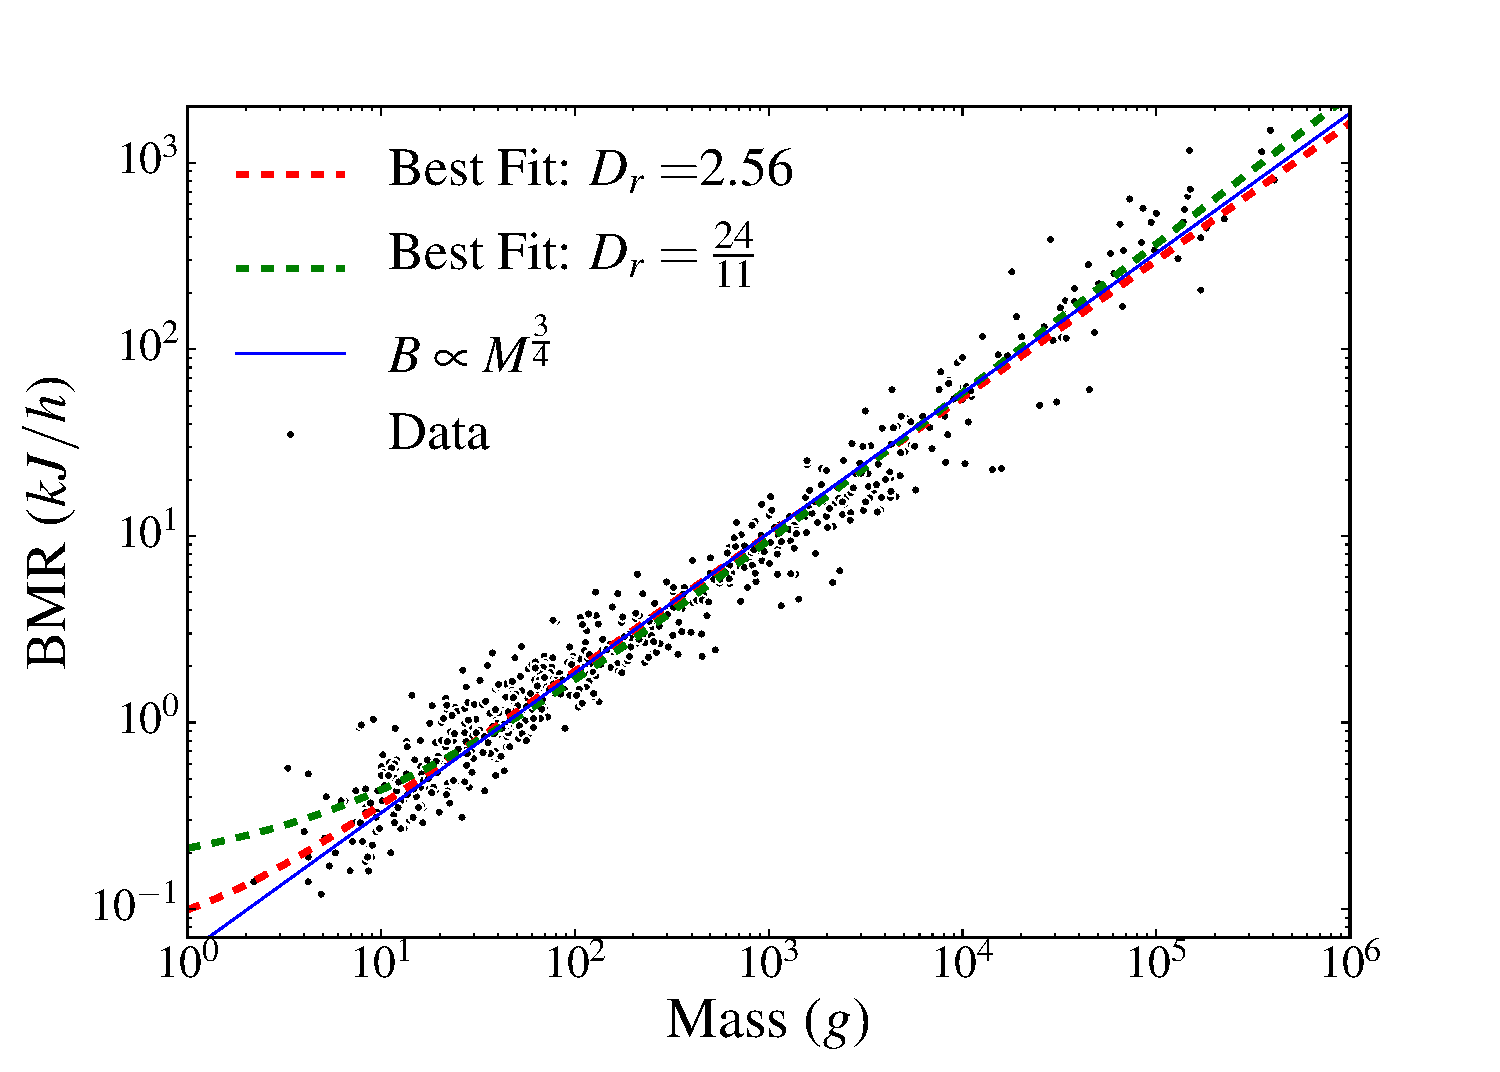
\includegraphics[height=70mm]{Figures/OrganismsPowerScalingv2.pdf}

  \caption{\red{The energy-time minimization model predicts metabolic
    scaling in mammals. Data from ~\cite{kolokotrones2010curvature}
    show slight, but theoretically important, curvature in the scaling of metabolic rate vs. mass of mammals.  The  theoretical optimum predicted by Eq.~\ref{eq:OrganismPower}
    with $D_r = \frac{24}{11}$ is shown as a solid blue line. The West et
    al. $3/4$ scaling prediction~\cite{west97} is shown as a dashed red line, and the best empirical fit of Eq.~\ref{eq:OrganismPower} to the data is
    shown as a dashed green line ($D_r = 2.50$).}}
\label{fig:OrganismsPowerScaling}
\end{figure}

% was fit to data from~\cite{kolokotrones2010curvature} by adjusting
%    $D_r$ to minimize the distance
%5    from the empirical points to the modeled curve (red dashed line).  


\subsection{Microprocessor Model}
\label{sec:computers}

We now apply the same reasoning to computer chips. 
In computers, unlike biology,  nodes (transistors) 
are not constant size but have shrunk by many orders of magnitude over 40
years of microarchitecture evolution.  \red{During this time, total chip area has grown
much more slowly, and we assume it to be constant for our
calculations.   In addition, the total area of all transistors on the
chip is a fixed fraction of the area of the chip \cite{moses08}. 
Putting these two constraints together, the linear dimensions of transistors
%and wires 
decrease with transistor count as $N^{-1/2}$ (more generally,
$N^{-1/D_l}$). } The width of the smallest wires is 
$r_0 \propto N^{\frac{-1}{D_l}}$ because minimum
transistor size and wire width are both determined by the process size.
Similarly $l_0 \propto  N^{\frac{-1}{D_l}}$ because transistor linear density
is increasing as $N^{\frac{1}{2}}$.
Intuitively, this means
that the number of nodes increases as smaller transistors are placed closer
together and connected with smaller and shorter wires. In the following,
we assume that all wires carry the same flow and that information is
transferred synchronously. We now calculate how $E_{net}$, $T_{net}$,
$E_{node}$ and $T_{node}$ scale with the number of transistors, $N$, and the three
scaling dimensions, $D_l$, $D_r$ and $D_w$.

$E_{net}$ can be calculated from basic principles of electronics as the energy
dissipated to transmit a bit over a wire: $\frac{CV^2}{2}$, where $C$ is
capacitance and $V$ is voltage.  Because $V$ has remained approximately
constant over the last four decades (decreasing only by a factor of five while
transistor count increased by six orders of magnitude \cite{ning07}), we
estimate that the total energy to transmit all bits over the network scales as
$C$ \cite{bingham08}.  Ignoring fringe effects and for an aspect ratio of 1,
wire capacitance is proportional to wire length, $C = \epsilon l$
\cite{wilhelm95}, where $\epsilon$ is the dielectric constant. Thus, the
network capacitance is the sum of the capacitances of all wires, which is
proportional to the total wire length of the network~\cite{donath79}:

\begin{equation}
  \label{eq:ChipsEnet}
  E_{net} \propto C \propto  \sum_{i=0}^H l_i w_i n_i \propto l_0 w_0 \lambda^H
\sum_{i=0}^H \lambda^{i \left( \frac{1}{D_l} + \frac{1}{D_w} -1  \right)} 
\end{equation}

\noindent where at all levels $i$, $l_i$ is the length of wire, $w_i$ is the number of wires per
module, and $n_i$ is the number of modules. Recalling that
$l_0 \propto N^{-1/D_l}$ and $\lambda^H \propto N$ gives: 
\begin{equation}
\label{eq:comp-Enet}
  E_{net}  \propto  N^{(1- \frac{1}{D_l})} \sum_{i=0}^H \lambda^{i \left( 
\frac{1}{D_l} + \frac{1}{D_w} -1 \right)} .
\end{equation}

\noindent Note that the scaling of $E_{net} $ with $N$ depends on $D_l$ and
$D_w$, but not on $D_r$. Similarly to energy scaling in
mammals, how $E_{net}$ scales depends on whether the exponent
$\frac{1}{D_l} + \frac{1}{D_w}-1$ in Eq. \ref {eq:comp-Enet} is positive or
negative.  If $D_w \geq \frac{D_l}{D_l -1}$ the exponent is negative and the
summand converges to a constant ($\log(N)$ in the case of exact equality),
leaving $E_{net} \propto N^{1-\frac{1}{D_l}}$. When $D_w < \frac{D_l}{D_l -1}$,
$C \propto N^{\frac{1}{D_w}}$. Given $D_l = 2$ for two-dimensional chips, $E_{net}$
is minimized when $D_w \geq 2$. See Section~\ref{sec:AppendixChips} for
details.

We now calculate the scaling of $E_{node}$ ignoring leakage
power.\footnote{\red{Transistors and other devices conduct a small amount
  of current even when they are not being used. This energy loss is referred
  to as leakage power and is a significant issue in modern
  microprocessor design not explicitly addressed by our model.}}
For a single node, computation
energy is given by the transistor's (dynamic) energy dissipation as
$\frac{CV^2}{2}$. Again assuming constant $V$ and the capacitance of a
transistor proportional to its length ($l_0$), $E_{node}$ is obtained
by summing
the capacitance across all $N$ nodes giving $E_{node} \propto N l_0  \propto
N^{1-\frac{1}{D_l}}$. 

We calculate $T_{net}$ as the time to transmit a bit over the last 
wire
in the network that connects to each transistor. This assumes perfect
pipelining so there is no delay in signal arriving at the last wire
(Appendix~\ref{sec:AppendixChips} shows that perfect pipelining requires $D_r =
2$). Thus, $T_{net}$ is equivalent to the wire latency which equals resistance
multiplied by the capacitance of the wire ($RC$). For wires with aspect ratio
1, $R_i = \rho l_i /r_i^2$, where $\rho$ is the resistivity of the material,
and $C_i \propto l_i$ as above.  Thus, 

\begin{equation}
\label{eq:comp-Tnet}
T_{net} \propto R_0C_0 \propto
\frac{{l_0}^2}{{r_0}^2} \propto N^0 .
\end {equation}
\noindent $ \frac{{l_0}^2}{{r_0}^2}$ is constant
because in chips  $l_0 \propto r_0$ and both are determined by process size.

Computation time for each node, $T_{node}$, is calculated as the transistor
delay, $\frac{CV}{I}$ ~\cite{bakoglu90}, where again $V$ is constant and $C$ is
proportional to transistor length: $T_{node} \propto C_0 \frac{V}{I}  \propto
l_0  \propto N^{-\frac{1}{D_l}}$. 

Before calculating the energy-time product, we observe that $T_{net}$ is the
only term that depends on $D_r$, so we set  $D_r = 2$ to minimize
$T_{net}$. Similarly, $E_{net}$ is the only term that depends on  $D_w$, and we
set $D_w$ to minimize $E_{net}$. \red{In summary, given $D_l = 2$, the terms of the energy-time product are minimized
when $D_r = 2$ and $D_w > 2$. Although
the energy-time product is minimized for values of $D_w$ greater than 2,
this would entail greater communication locality, which is challenging
to engineer and doesn't improve
the energy-time product.  Thus, the model predicts 
that $D_w = 2$, which is consistent with observed
Rent's exponents that approach 1/2~\cite{yang2001wirelength, solee2013evolutionary}.}  The scaling relations for various
quantities are summarized in Table~\ref{tab:Predictions}.

\subsection{Predictions for Microprocessors}
\label{sec:comp-predictions}

\red{Summarizing the results from the previous section, the energy-time
product for chips is minimized when 
$D_l=D_r =2 =D_w$.}
This result corresponds to ideal scaling, as suggested by Dennard
\cite{dennard74}, where the linear dimensions of transistors and wires scale at
the same rate, wire delay is constant, and the Rent's exponent is 1/2.  

The final energy-time product scales as $N^{1/2}$ \red{(Table \ref{tab:Predictions}}), showing that, unlike
mammals, as size increases, the energy-delay product per node decreases
systematically.  Thus, chips have become faster and they consume less energy per
transistor as more transistors are packed onto a chip. Of course, this
trend \red{arises}
from the remarkable miniaturization of transistors and wires described by
Moore's law. It is not surprising that transistors are faster ($T_{node}$) and
require less energy ($E_{node}$) as they become smaller. It also makes sense
that  $E_{net}$ grows sub-linearly with the number of transistors, because as
$N$ increases the distance between nodes is reduced. Additionally, $D_w = 2$,
means that most bits move locally, so the distance between nearest nodes
affects the average distance that bits are transmitted.  The only term in the
energy-time product that does not decrease with increased $N$ and decreased
process size is $T_{net}$ which remains constant under Dennard scaling where
wire radius and length scale proportionally to each other.

These scaling models make two testable predictions.  First, power
consumption ($P$) in chips (total energy dissipated per unit of time) scales as

\begin{equation}
\label{eq:Power}
P = \frac{E_{sys}}{T_{sys}} \propto N^{1/2} .
\end{equation}
 
\noindent Second, performance,
measured as computations executed per unit of time, or throughput ($Tp$), is predicted
to scale linearly with $N$,  i.e.  

\begin{equation}
\label{eq:Performance}
Tp\propto \frac{N}{T_{sys}} \propto N .
\end{equation}

We compared our theoretical predictions for active power consumption (ignoring leakage power as discussed above) with data
obtained for 523 different microprocessors over a range of approximately 6
orders of magnitude in transistor count (See section~\ref{subsec:chipdata} for
details of the data collection).  The data are shown in
Figure~\ref{fig:power}, where the measured exponent was $0.495$ (95\%
confidence interval = 0.46 to 0.53) which agrees closely with our prediction of
$0.5$. Consistent data on performance across many technology generations is
difficult to obtain because reporting standards have changed over the years and
their adoption by different vendors is not uniform.  \red{We obtained
normalized performance data for 100 different Intel chips, measured
with \red{Dhrystone} Millions of Instructions per Second (DMIPS), from
a variety of sources (see Section \ref{subsec:chipdata}).} These sources included
a variety of published third-party performance comparisons from different
generations over a range of 6 orders of magnitude in transistor count.  The
best-fit exponent for these data is $1.11$ (95\% confidence interval =1.07 to
1.15), as shown in Figure~\ref{fig:throughput}. This is close to our
predicted exponent of $1$, suggesting that engineered designs slightly
outperform the theoretical optimum defined by the model. Performance and throughput were fit
using least squares regression, assuming that there
are no significant errors in the reported count of the number of transistors~\cite{mcardle1988structural}.  

It is somewhat counter-intuitive that
performance increases only linearly with the number of transistors.
Given that transistor switching times have decreased
dramatically as size has decreased, one might expect performance to increase as
the product of clock speed and transistor number ($N$).  However, this
is not the case, and we show
the expected performance if time were actually the inverse of clock
speed in the red dotted line in Figure~\ref{fig:throughput}. Some performance
increases are achieved by increasing clock speed for a given manufacturing
process, which may account for the higher than predicted scaling
exponent\footnote{Additionally, higher end chips are more likely to be
benchmarked, potentially leading to a bias in the data towards higher
performing chips.}. This analysis confirms that the network is indeed the
bottleneck. The network delivers bits to transistors at a constant rate per
transistor (Eq. \ref{eq:comp-Tnet}), so performance has increased only linearly
with transistor number even though, in principle, smaller transistors could process
information more quickly.  As in biology, performance cannot be understood
without considering the constraints of the network.


\begin{figure}[!h]
\centering
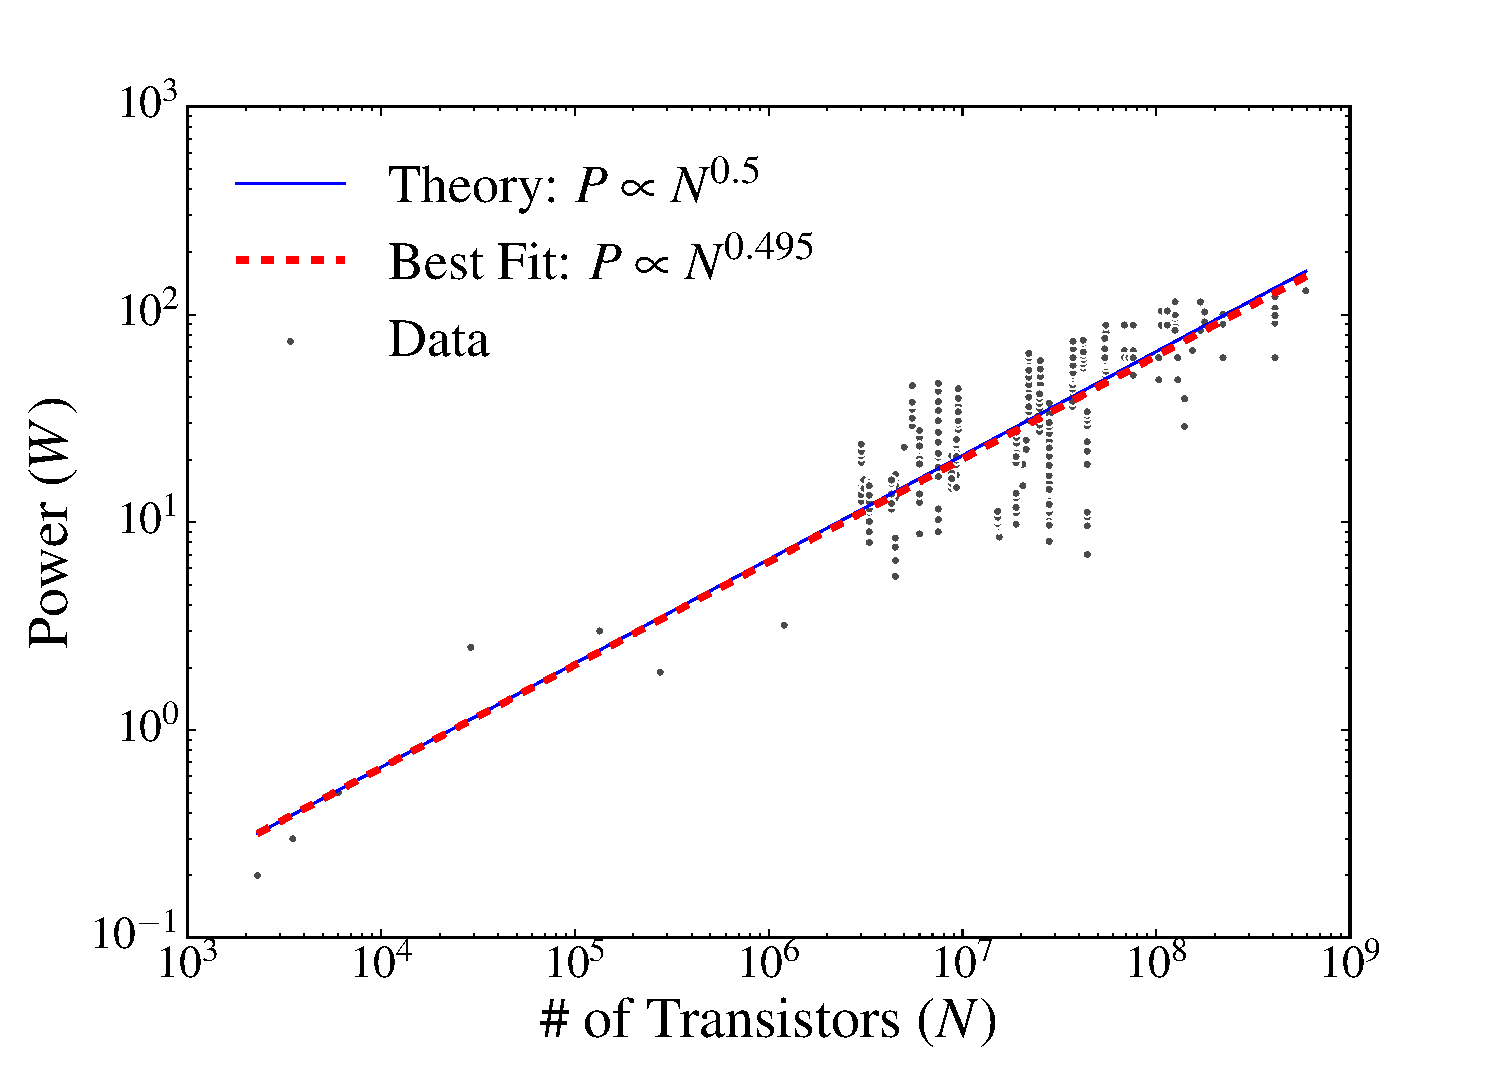
\includegraphics[height=70mm]{Figures/ChipsPowerScaling.pdf}
\caption{\red{The energy-time minimization model predicts power
scaling in chips. Each data point represents a microprocessor chip, with active power and number of transistors per chip from \cite{moses08}.  The energy-time minimization model
prediction (Eq. \ref{eq:Power}) is shown in blue, and the best fit line is shown in green.}}
\label{fig:power}
\end{figure}

\begin{figure}[!h]
\centering
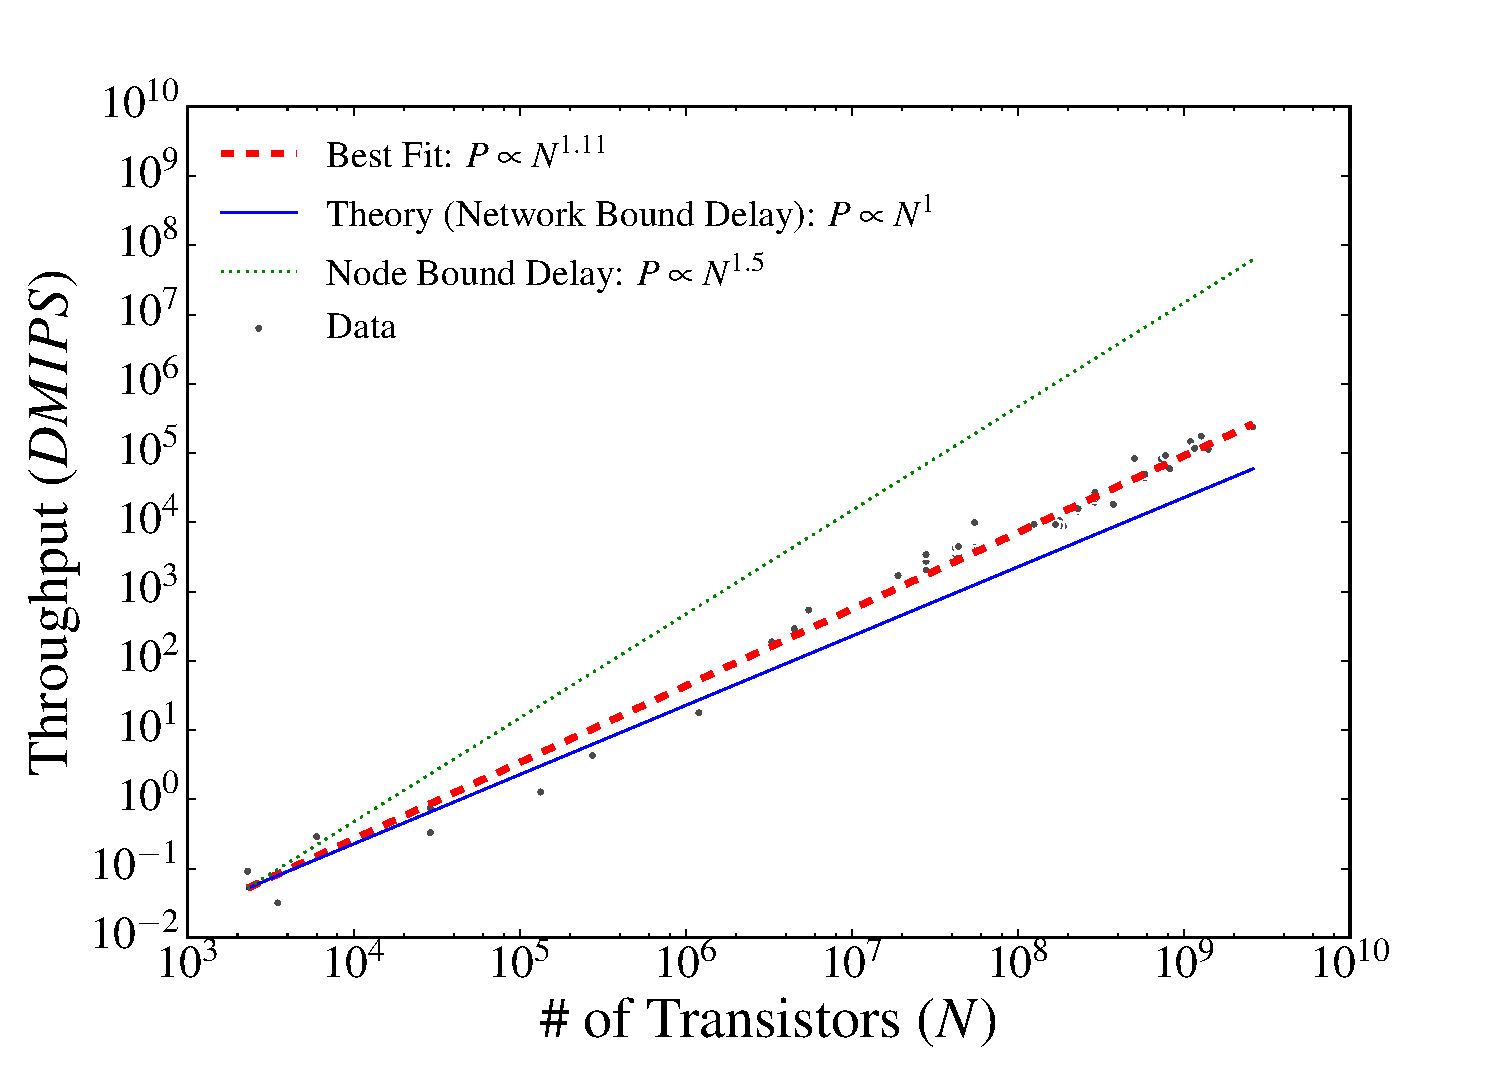
\includegraphics[height=70mm]{Figures/ChipsThroughputScaling.pdf}
\caption{\red{The energy-time minimization model predicts how throughput
  scales with the number of transistors.  The raw data and their sources are included as
  supplementary material. The model
 prediction  (Eq. \ref{eq:Performance}) is shown as a solid blue
  line. The dotted red line shows an alternative prediction if throughput were 
  bound by the nodes (switching speed) rather than the network. The
  green dashed line is the best fit to the data.}}
\label{fig:throughput}
\end{figure}

Our model provides a simple theoretical explanation for the scaling of power
and performance in computers over 40 years of microprocessor technology
improvements.  The excellent agreement between the theoretical optimum and
experimental data suggests that through successive generations of
trial-and-error, innovation and optimization, engineered designs are highly
successful, approaching and sometimes exceeding the theoretical optimum predicted by the model.


\section{Discussion}
\label{sec:discussion}

\subsection{Summary of scaling predictions}
Scaling analyses provide a framework for understanding critical
parameters and constraints on the design of both biological and
computational systems spanning an enormous range of sizes.   We have
presented a unified model which predicts scaling relationships for both mammals and
microprocessors by simultaneously minimizing energy dissipation and delivery time. 
%gives
%unified model, accounting for how both natural and artificial
%networks have evolved. 
The energy-time minimization model highlights the similarities and
differences between biological networks that deliver oxygen and
computational networks that deliver information.  \red{Earlier scaling
models focus either on minimizing energy dissipation or on minimizing
delivery time, e.g., \cite{west97,banavar10}.  Here we extend that work by considering minimization of energy and time
simultaneously and investigating the tradeoffs between them.}

\red{This theoretical model makes testable scaling predictions for biological metabolism and for the power and performance of computers.  In biology, Section
\ref{sec:bio-predictions} extends previous predictions to explain the
observed curvature in metabolic scaling of mammals.  \red{Other studies have interpreted the
deviation from linear scaling as indicating that there is no single unified metabolic scaling theory, for example as imperfect matching of supply and demand~\cite{banavar2002supply}. The
framework presented here accounts for curvature in the optimization model by including both time and energy minimization in both the network and the nodes.} In computation, the unified model accurately predicts Rent's exponents, active power consumption and chip performance in over 40 years of chip design.
%The model is consistent with the results of a
%previous study~\cite{delong2010shifts} at the evolutionary transitions. 
Thus,
the model provides evidence of strong convergence between natural and
engineered designs due to physical constraints despite the obvious
differences between them.} 
%These
%results might be useful when understanding the emergence of sociality
%and the transition to complex animal societies.

The model presented here is, of course, a simplification of the more
complex reality. For example, our analysis assumes that $D_l$, $D_r$,
and $D_w$ are fixed constants throughout the network both within and
across systems. In reality, each of these may vary.  For
example,~\cite{newberry2015testing} did not find evidence for a
constant $D_l = 3$ in mouse vasculature, suggesting that the network
does not deliver resources uniformly throughout the body volume. This
is not surprising given that different tissues and organs have
different metabolic requirements. $D_r$ may vary
within the vascular network with area-preserving branching closer to the heart and area-increasing branching slowing blood velocity in smaller
vessels, but~\cite{newberry2015testing} find values for $D_r$
consistent with our predictions.  Similarly, there is evidence that
$D_w$ varies across hierarchical levels in computer
chips~\cite{ozaktas2004information}. Including these factors in the
model would allow more accurate predictions, but they are unlikely to
substantively change the order-of-magnitude predictions of 
our simple unified model.

Our model makes novel predictions both for mammals and
microprocessors. For mammals we give the first quantitative prediction
for $D_r$ that accounts both for blood slowing through the network and
for the empirically observed curvature in scaling relations that cause
small and very large mammals to deviate from $3/4$ scaling predictions. Additionally, 
this prediction ($D_r = \frac{24}{11}$) gives an energy-time product that is approximately linear with $N$ ($E_{sys} \propto N^{1/12} + N^1$, Table 1). Highlighting the inherent tradeoff between energy dissipation and delivery times 
has important implications for understanding the energetic basis of fitness.  Some have proposed that biological fitness
maximizes metabolic power (energy/time) \cite{lotka56, odum71}, whereas others
have proposed that it minimizes biological times (e.g., generation times, which
is equivalent to maximizing vital rates) \cite{lindstedt81, sibly91}. The
invariance of the energy-time product on a per-node basis is
consistent with the idea that organism fitness
is largely independent of body mass.  Mammals of all sizes, from
small, fast, low-power mice to large, slow, powerful elephants, coexist and,
therefore, are likely nearly equally fit.  This implies a direct trade-off
between maximizing metabolic power and minimizing generation times, which holds
over the many orders-of-magnitude variation in body mass.  The energy-time
product reflects powerful geometric, physical and biological constraints on the
evolution of organism designs.

In computation, the model accurately predicts power consumption and
performance of computer chips as simple functions of the number of
transistors. These order-of-magnitude performance predictions highlight that delivery of
bits through the network, rather than processing bits at the
transistors, is the rate limiting step that constrains performance.
More precise predictions may be obtained by incorporating additional
factors, for example leakage power, which comprises an increasing fraction
of the power budget of computer chips~\cite{horowitz2005scaling}.

\subsection{Implications for Evolutionary Transitions}

The similarities between biological and computational scaling suggest
future trajectories in computing based on how the fundamental
structural and functional properties of organisms from bacteria to mammals have changed over
evolutionary time. Work by Delong et
al.~\cite{delong2010shifts} demonstrated that the slopes and
intercepts of metabolic scaling relations change at the evolutionary
	transitions: prokaryote (bacteria) metabolic rate varies \emph{superlinearly}
with size, unicellular protist rate varies  \emph{linearly}, and
whole-organism metabolic rate of multicellular animals scales
 \emph{sublinearly}, converging to the canonical $3/4$ exponent that approximates the mammalian scaling described above. They
hypothesize that these discontinuous scaling shifts arise from body plans
overcoming pre-existing constraints, and then accommodating to new
constraints, as body size and complexity increase.

Delong et al. hypothesize the following: Larger bacteria have higher metabolic rates because their larger genomes allow increased use of
metabolic substrates, but eventually cell surface area limits metabolic
processing. Unicellular protists overcome this constraint by internalizing the metabolic machinery into
respiratory organelles (i.e., mitochondria that convert oxygen into ATP). The
number of mitochondria increases linearly with cell size until intracellular
transport constraints begin to limit the rate of metabolic processing.
Next, multi-cellular
animals have effectively invariant cell size and intracellular transport, but as as body size and number of cells increased, vascular networks evolved to rapidly and efficient deliver metabolites. However, vascular networks introduce the sublinear network scaling effects characterized above. 

Delong et al. highlight the
importance of both time and energy constraints, and these change at each evolutionary transition, with the consequence that the absolute time and quantity of
energy required to deliver each molecule of oxygen increase across the major evolutionary transitions. \red{This suggests that the energy-time minimization framework which we have used to predict the curvature in metabolic scaling in mammals, might be also be applicable across the full range of living organisms, with different constraints on time and energy emerging at each evolutionary transition.} The explanations that they hypothesize are also directly relevant
to understanding how energy-time minimization affects the ongoing evolution of
computer hardware.

\red{\subsubsection{Innovations in chip design mimic innovation in the evolution of bacteria}} The chip scaling described above
shows how time and energy dissipation have decreased while performance
increased as larger numbers of smaller transistors have been packed
onto each chip. During this era, technological innovations in chips
have emerged that optimize against physical constraints.  Just as
bacteria have evolved larger genomes and used the new genes to exploit
new metabolic niches, new materials, switching methods, etching
processes and cooling technologies have pushed physical boundaries,
allowing transistors to shrink and more of them to be packed onto each
chip. Like bacteria, however, there are limits to this process.  There are no elephant-sized bacteria, and there will be no
silicon-based single core chips with quadrillions of transistors.

\red {\subsubsection{Single core chip scaling mimics unicellular protists}} Historical chip scaling mimics the linear relationship between performance and
size (Figure \ref{fig:throughput}) seen in protists. Unicellular protists show linear increases
in metabolic rate with size (Figure 1 of reference~\cite{delong2010shifts}) as more energy processing nodes (mitochondria) are
packed into larger cells. As size continues to increase however, this
design strategy also reaches physical limits.  Our analysis suggests that the
internal transport network already constrains processing speeds
($T_{net}$ constrains $T_{sys}$). Further, the requirement to
dissipate heat over a fixed surface area constrains both cells and chips. 

\red{\subsubsection{Multi-core chips echo the transition to multicellularity}} Computer chips are currently undergoing
the evolutionary transition to multicore, resembling the biological
transition to multicellularity. Our unified scaling framework suggests
some future scenarios. As the era of transistor minimization wanes,
additional transistors will require increased physical area, and
therefore networks that span greater distances. Similar to
multicellular organisms, we expect that as the number of cores grows,
an increasing fraction of chip power will be devoted to these ever
larger Networks-on-Chip (NoC) connecting more cores. Larger networks
will consume more power, take more time to traverse, and ultimately
the time-energy minimization will be increasingly difficult to sustain
as chips increase in size.  Clock speeds have already leveled off as 
power, footprint and
cooling requirements 
%of the network 
dominate chip design
considerations~\cite{waldrop2016chips}.  If chips follow biology, we can expect
that the most important future advances in chip
design will increase network efficiency, for example by using optical
networks.

\red{\subsubsection{Computer scaling deviates from biological scaling in important ways}} There are also important differences between scaling of oxygen delivery in biology and information
delivery in computation, which play an important role in evolutionary
transitions. In particular, on-chip computer networks have two advantages not
available to cardiovascular networks.  First, the shrinking of
`process' size (smaller
transistors and wires) reduces both energy and
delay in the nodes as the number of nodes increases.
This reduction in process size will ultimately end
as physical limits are reached~\cite{waldrop2016chips}.
Second, the locality of
network traffic, characterized by the Rent's exponent and $D_w$, reduces long
distance communication over computer networks. As shown above, this
effect
reduces $E_{net}$ and leads to a smaller wire footprint as $N$
increases on single core chips. This advantage will likely continue for
multi-core chips where communication, and therefore network bandwidth,
footprint and energy consumption of NOCs can be reduced by keeping
communication primarily local~\cite{bezerra2010modeling, zarkesh2010hybrid}. Communication locality
has the potential to produce more favorable scaling in multi-core
computation than is achievable in multicellular biology.

\red{\subsubsection{Decentralized designs in the transition to sociality}}  We now
consider how the lessons learned from computer architecture may lend insights into an important
biological evolutionary transition, the transition to social animal societies. Understanding and improving the flow of energy, materials and information through human societies is one of the greatest challenges facing science and engineering, and scaling analyses lend an important perspective on this problem~\cite{moses2012beyond}.
Sociality is an important evolutionary transition, reflected in the
ecological dominance of humans and ants whose networked
systems transport both energy and information. These social species have experienced great success, dispersing over vast territories across the globe and capturing a large
fraction of available energy ~\cite{haberl2007quantifying, holldobler1990ants}. Recent evidence suggests that ant colonies and human societies follow similar scaling relationships as individual organisms~\cite{moses2003allometry, bettencourt2007growth, burnside2012human, hou2010energetic, waters2010allometric}. 

In social animal systems and networked computer systems, networks
are at least partially decentralized, for example traffic flow within cities~\cite{samaniego2008cities} and among ant nests~\cite{flanagan2013fast}. Tainter et. al.~\cite{tainter2003resource} argue that complex human and ant societies are able to exploit ``low-gain'' energy systems: those that provide low concentrations of dispersed energy, but that are ubiquitous and therefore can be exploited by complex systems capable of processing and storing vast quantities of energy. Understanding the forces that have driven the tremendous power and performance scaling in computing may lend insights into how other technologies exploit similar scaling relationships~\cite{buchanan2016generalizing}. In particular, communication locality in computation suggests an important strategy in the transition to sociality: animal societies can escape the constraints of the centralized distribution network
by evolving systems for decentralized transportation and modular communication. Indeed, the transition to solar energy is capitalizing on the same kind of dramatic technological performance improvements that computer technology experienced as Moore's Law~\cite{farmer2016predictable}.  The history of computing suggests large gains in the efficiency of energy delivery if increasingly powerful solar cells utilize dispersed solar energy locally to escape the centralized distribution overhead of the fossil fuel based economy.
 
 Moreover, power laws as a function of size are not
unique to organisms and computers but are observed across a wide
variety of complex systems in nature, society and technology.  \red{The scaling of
white and grey matter~\cite{zhang00} and communication modularity~\cite{meunier2010modular} in the brain, of flow through river networks that minimize transportation costs~\cite{banavar2000topology}, of energy use and GDP in
countries \cite{brown11}, and the pace of life and population in cities
\cite{bettencourt07} are all additional examples that a unifying scaling theory might explain.}  Because cost and performance, i.e., energy and time, impose
universal constraints, we suggest that a common design principle may govern the
scaling of many evolved and engineered complex systems that process energy, materials and information.

\vspace{10 mm}
\section{Conclusion}

Our analysis provides a unifying explanation for the origin of scaling laws in
biology and computing. Despite obvious differences in form and function, the
scaling of organisms and computers is governed by the same simple principle: minimizing the energy and time to deliver and process resources. Both natural selection and human engineering have evolved designs that manage the trade-off between cost and performance to minimize energy dissipation and time to deliver resources, resulting in general scaling laws that predict metabolic rate, and microprocessor power and performance over several orders-of-magnitude variation in system size. 

Engineering ingenuity and economic pressures have created increasingly
fast and powerful computers through a series of innovations, including
integrated circuits, innovations in materials and other technological
tricks, synchronizing clock trees, multi-core chips and networked and
distributed computation. Today, technology is undergoing another
major evolutionary transition as distributed computing changes the
metabolic landscape of technology that is becoming more tightly coupled with the
environment. As computers are embedded in more physical devices,
physical proximity and energy concerns for low-power devices may drive
computational scaling to more closely resemble biological scaling. In
computation, dramatic changes have emerged over the last 35 years, but
to a surprising extent, their trajectories mimic the biological
transitions that took billions of years to evolve simple unicellular
bacteria into the largest and most powerful animals and societies on
earth.


\newpage

\section{Appendix A: Details of Scaling in Organisms}
\label{sec:AppendixOrg}

This appendix gives the full derivation of the scaling equations.  We
begin with the total network resistance discussed in
Section~\ref{sec:mammals}, and its subsequent effect on the energy
time product scaling. Assume that $D_l = 3$ for $3$ dimensional
organisms and that $\lambda^{-H}=N^{-1}$.  Using these values and
simplifying, equation~\ref{eq:resistance} is transformed.

\begin{equation}
 R = \frac{8 \mu l_0}{\pi r_0^4} N^{-1} \sum_{i=0}^H \lambda^{i(\frac{4}{3} -\frac{4}{D_r})}
\end{equation}

Let the summand $S = \sum_{i=0}^H \lambda^{i(\frac{4}{3} -\frac{4}{D_r})}$. $R \propto
N^{-1} S$. How $S$ scales with $N$ is dependent on the exponent $\frac{4}{3} -
\frac{4}{D_r}$, and reduces to three different cases:

\begin{caseof}

    \case{$D_r=3$}{In this case the exponent is equal to 0, and the $S = H+1
      \propto \log (N)$, and $R\propto \frac{\log(N)}{N}$, because $\log(N)$
      in this case grows much more slowly than $N$, it is reasonable to
      conclude that $R\propto N^{-1}$. In this case the energy time product
      scales as $l_0 + u_0^{-1}N^{2-\frac{2}{D_r}}$.}

    \case{$D_r < 3$}{Here (and in subsequent cases) we can use the geometric
      series to calculate the exact value of $S$. In particular 

      \begin{align*}
        S &= \frac{(1-\lambda^{(\frac{4}{3}
    -\frac{4}{D_r})(H+1)})}{1-\lambda^{\frac{4}{3} -\frac{4}{D_r}}} \\ 
        &= \frac{1-\left(\lambda^{H}\right)^{(\frac{4}{3}-\frac{4}{D_r})}
      \lambda^{(\frac{4}{3} - \frac{4}{D_r}))}}{1-\lambda^{\frac{4}{3}
      -\frac{4}{D_r}}} \\
        &= \frac{1-N^{(\frac{4}{3}-\frac{4}{D_r})}
      \lambda^{(\frac{4}{3} - \frac{4}{D_r}))}}{1-\lambda^{\frac{4}{3}
           -\frac{4}{D_r}}}
      \end{align*}

      If we let $c = \lambda^{(\frac{4}{3} -\frac{4}{D_r})}$ we see that

      \begin{equation}
        S = \frac{1-c N^{(\frac{4}{3}-\frac{4}{D_r})}}{1-c}
      \end{equation}

      Because $\frac{4}{3} - \frac{4}{D_r} < 0$ is negative in this case
      and $N$ is large in practice, $c N^{(\frac{4}{3} -\frac{4}{D_r})}$ is
      small, and $S$ is proportional to a constant ($S \approx
    \frac{1}{1-c}$). This implies that $R \propto N^{-1}$. Once
  again, equation~\ref{eq:TheWholeEnchilada} scales as $\propto l_0 +
u_0^{-1}N^{2-\frac{2}{D_r}}$.}

    \case{$D_r >3 $}{In this case the exponent in $S$ is positive,
      meaning that $S$ scales directly with $N$. Note that $c>1$ in this case
      and we can write 
      \begin{equation}
        S = \frac{c N^{(\frac{4}{3}-\frac{4}{D_r})}-1}{c-1}
      \end{equation}

      \noindent This means that $S \propto N^{(\frac{4}{3} - \frac{4}{D_r})}$.
      This implies that $R \propto N^{-1} S \propto N^{(\frac{1}{3}
      -\frac{4}{D_r})}$. This means that resistance still scales inversely with
      size, but at a faster rate than if $D_r \leq 3$. This implies the energy
    time produce scales as $\propto N^{\frac{4}{3} - \frac{4}{D_r}} +
  N^{2-\frac{2}{D_r}}$. Note that this results in a positive scaling of $R$ with $N$ if $D_r>12$. }


\end{caseof}

\subsection{Length, Velocity and Mass Scaling}
\label{subsec:appendixLengthMass}

We determine the scaling of $l_0$, $u_0$ and $M$ following the method 
presented in Banavar et al.~\cite{banavar10}. Specifically, we assume that $M
\propto V \propto V_{net}$, where $V$ is the volume of the organism, $V_{net}$ is the volume of the network
transporting oxygen molecules, and

\begin{equation}
u_0 \propto l_0 \propto \left (\frac{V}{N} \right) ^{\frac{1}{3}}
\end{equation}

We calculate $V_{net}$ as: 

\begin{align*}
V_{net} &= \sum_{i=0}^H V_i = \sum s^{-1} l_i r_i^2 n_i \\
  &= \sum_{i=0}^H {l_0}^{-1} l_0 \lambda^{\frac{i}{D_l}} r_0^2 \lambda^{\frac{2i}{D_r}}
  \lambda^{H-i} \\
  &= \lambda^H r_0^2 \sum_{i=0}^H \lambda^{i \left(\frac{i}{D_l} +
  \frac{2}{D_r} - 1 \right) } \\
  &\propto N^{\frac{1}{D_l} + \frac{2}{D_r}} 
\end{align*}

Note that $s \propto l_0$ is the linear distance between oxygen molecules that will be delivered to the same capillary, allowing narrower vessels when oxygen travels at higher velocity (see ~\cite{banavar10} Figure 3 for further explanation). The calculation assumes that $\frac{1}{D_l} + \frac{2}{D_r} -1 > 0$ which
will always be the case with $2 < D_r < 3$, and $D_l=3$. 

Therefore $M\propto N^{\frac{1}{D_l} +
\frac{2}{D_r}}$,
and $N \propto M^{\frac{1}{\frac{1}{3} + \frac{2}{D_r}}}$, where $D_l=3$.
Additionally

\begin{align*}
u_0 \propto l_0 & \propto \left( \frac{V}{N} \right)^{\frac{1}{3}} \\
    & \propto \left( N^{\frac{1}{3} + \frac{2}{D_r} - 1} \right)^{\frac{1}{3}} \\
    & \propto N^{\frac{2}{3D_r} - \frac{2}{9}}
\end{align*}

Combining these results with $E_{sys}$ and $T_{sys}$ in
Table~\ref{tab:Predictions}, we derive how metabolic rate, $B$
(measured in power), scales with the mass of an organism.

\begin{align*}
B = \frac{E_{sys}}{T_{sys}} =& \frac{RQ^2}{N} + Q \\
 \propto & u_0^2 l_0 N^{-2} N^{\frac{4}{D_r}} + u_0 N^{\frac{2}{D_r}} \\
 \propto & N^{\frac{6}{D_r}- \frac{8}{3}} + N^{\frac{8}{3 D_r} - \frac{2}{9}} \\
 \propto & M^{\frac{\frac{6}{D_r} - \frac{8}{3}}{\frac{2}{D_r} + \frac{1}{3}}}
 + M^{\frac{\frac{8}{3D_r} - \frac{2}{9}}{\frac{2}{D_r} + \frac{1}{3}} } \\
 \propto & M^{\frac{18-8D_r}{6+Dr}} + M^{\frac{24-2D_r}{18-3D_r}} 
\end{align*}

\newpage

\section{Appendix B: Details of Scaling in Electronics}
\label{sec:AppendixChips}

In this section we give a detailed analysis of the derivation of the scaling of
the network capacitance and network latency discussed in
Section~\ref{sec:computers}.

\subsection{Capacitance}

Recall that $D_l = 2$ for $2$ dimensional computer
chips and that $\lambda^{-H}=N^{-1}$. We can then calculate capacitance as:

\begin{equation}
  C \propto  N^{(1- \frac{1}{D_l})} \sum_{i=0}^H \lambda^{i \left( 
\frac{1}{D_l} + \frac{1}{D_w} -1 \right)}
\end{equation}

Similar to how we handled organsims we are interested in whether the exponent
$\frac{1}{D_l} + \frac{1}{D_w} -1$ is positive or negative.

Let the summand $S = \sum_{i=0}^H \lambda^{i(\frac{1}{D_l} +
\frac{1}{D_w}-1)}$. $C \propto
N^{1-\frac{1}{D_l}} S$. 

\begin{caseof}

  \case{$D_r=\frac{D_l}{D_l-1}$}{In this case the exponent is equal to 0, and the $S = H+1
    \propto \log (N)$, and $C\propto \log(N) N^{1-\frac{1}{D_l}}$, because $\log(N)$ in
    this case grows much more slowly than $N^{1-\frac{1}{D_l}}$ and we know
    $D_l=2$ for 2 dimensional chips, it is reasonable to conclude that
  $C\propto N^{\frac{1}{2}}$}

  \case{$D_r > \frac{D_l}{D_l-1}$}{Here (and in subsequent cases) we can use
    the geometric series to calculate the exact value of $S$, using a similar
  approach to~\ref{sec:AppendixOrg}. In this case the exponent is negative and $S$
is a small constant, leaving $C \propto N^{\frac{1}{2}}$}

\case{$D_r < \frac{D_l}{D_l-1} $}{In this case the exponent in $S$ is positive,
      meaning that $S$ scales directly with $N$. Now the summand contributes an
    $N^{\frac{1}{D_l}+\frac{1}{D_w} -1}$ and $C \propto N^{\frac{1}{D_w}}$.}

\end{caseof}

\subsection{Network Delay}

Recall that we wish to determine the network latency $L$ which is defined as:

\begin{equation}
  T_{net} \propto \max_{i} L_i
\end{equation}

\noindent with

\begin{equation}
  L_i \propto RC = \frac{\rho \epsilon li^2}{r_i^2} = \frac{\rho \epsilon
  l_0^2}{r_0^2} \lambda^{i\left(\frac{2}{D_l} - \frac{2}{D_r}\right)}
\end{equation}

\noindent $L_i$ will scale differently depending on the relative values of
$D_r$ and $D_l$. 

\begin{caseof}

  \case{$D_r>D_l$}{In this case the fraction in the exponent is greater than 0
  and the latency will be highest when $i=H$, resulting in $L \propto
N^{\frac{2}{D_l} - \frac{2}{D_r}}$. }
  
  \case{$D_r <  D_l$}{In this case the exponent is negative and the highest
  latency occurs at the bottom of the network $i=0$, leaving $L\propto
\frac{l_0^2}{r_0^2} \propto N^0$}

  \case{$D_r = D_l$}{In this case the exponent is 0 and there is equal latency
  at all levels and $L \propto N^0$.}
\end{caseof}

\subsection{Chip Data}
\label{subsec:chipdata}

We obtain data on chip power usage and throughput from several third party
sources. For power output we consulted two web archives of over 523 chips
listing power consumption and transistor count~\cite{chipsPower1,chipsPower2}.
When possible the figures were cross checked with data directly from the
manufacturer. For throughput data, we consulted a combination of third party
sources, starting with a list published on wikipedia~\cite{wikiMIPS}. Each
source for the data was consulted independently and verified before inclusion
in the dataset. Additional throughput data was obtained from benchmarks
performed by online technology publication Tom's Hardware~\cite{tomsBenchmark}.
The data can be found in the supplementary information.

\newpage

\bibliography{references}
\bibliographystyle{abbrv}



\end{document}



